\documentclass[10pt,a4paper]{article}

\usepackage[margin=18mm,headheight=14pt]{geometry}
\usepackage{amsmath,amssymb}
\usepackage{booktabs,tabularx,array}
\usepackage{graphicx}
\usepackage{float}
\usepackage{xcolor}
\usepackage{fancyhdr}
\usepackage{tikz}
\usetikzlibrary{arrows.meta,positioning}
\usepackage[hidelinks]{hyperref}
\usepackage{fontspec}

\setmainfont{TeX Gyre Pagella}
\setsansfont{TeX Gyre Heros}
\setmonofont{Latin Modern Mono}

\definecolor{navy}{HTML}{16324F}
\definecolor{blue}{HTML}{1B6CA8}
\definecolor{teal}{HTML}{168A83}
\definecolor{orange}{HTML}{D97706}
\definecolor{red}{HTML}{B83A3A}
\definecolor{green}{HTML}{287A4B}
\definecolor{lightblue}{HTML}{EDF6FC}
\definecolor{lightorange}{HTML}{FFF5E8}
\definecolor{lightgreen}{HTML}{EEF8F1}
\definecolor{lightgray}{HTML}{F4F6F8}

\setlength{\parindent}{0pt}
\setlength{\parskip}{4pt}
\setlength{\emergencystretch}{3em}

\pagestyle{fancy}
\fancyhf{}
\lhead{SPECTRA-Siam}
\rhead{Five-minute executive summary}
\cfoot{\thepage}
\renewcommand{\headrulewidth}{0.4pt}

\newcommand{\R}{\mathbb{R}}
\newcommand{\code}[1]{\texttt{#1}}

\newenvironment{summarybox}[2]{%
  \begin{center}\begin{minipage}{0.95\linewidth}
  \colorbox{#1}{\parbox{0.96\linewidth}{\textcolor{navy}{\textbf{#2}}\par\smallskip}}
  \vspace{-6pt}\begin{quote}
}{\end{quote}\end{minipage}\end{center}}

\begin{document}

\begin{center}
{\LARGE\bfseries SPECTRA-Siam Method Evolution}\\[2mm]
{\large A five-minute summary of the architecture, failure, redesign, and results}\\[2mm]
{\small August 15, 2026}
\end{center}

\begin{summarybox}{lightgreen}{Bottom line}
The first spectral-only redesign failed because it compressed all semantic
information into the eigenvalues of a learned adjacency matrix. The second
redesign keeps canonical and lexical node information, but only as signals
processed by filters on the learned latent graph. It removes the disputed
direct feature bypass and recovers strong performance: on AtCoder it reaches
F1=0.832, Accuracy=0.824, Macro-F1=0.823, and ROC-AUC=0.893.
\end{summarybox}

\section*{1. Why the method had to change}

The legacy model combined three information routes:
\begin{enumerate}
\item a learned latent graph and its spectral descriptor;
\item a direct pooled representation of latent node states, $\operatorname{mean}(Z)$;
\item in the source-lexical configuration, a direct residual from source tokens.
\end{enumerate}
Canonical and node-level lexical features therefore helped construct the graph,
but also reached the classifier through a non-spectral path. Strong legacy
scores proved that the hybrid system worked; they did not prove that the
learned graph spectrum caused the improvement.

\begin{table}[H]
\centering
\small
\begin{tabularx}{\linewidth}{p{0.23\linewidth}XXX}
\toprule
Version & What reaches the classifier? & Methodological status & Observed behavior \\
\midrule
Legacy hybrid & Spectrum, pooled latent states, optional source residual & Attribution is ambiguous & Strong historical scores \\
First redesign & Eigenvalue density and heat trace only & Clean but overly restrictive & Representation collapse \\
Second redesign & Spectrum and energies of filtered graph signals & Spectral with no direct bypass & Strong, non-collapsed result \\
\bottomrule
\end{tabularx}
\caption{The three distinct architecture families.}
\end{table}

\begin{summarybox}{lightorange}{Important terminology}
The revised model is not eigenvalue-only. The correct label is
\emph{attributed latent graph-spectral representation} or
\emph{latent graph-signal spectral representation}.
\end{summarybox}

\clearpage
\section*{2. The revised architecture in one page}

Each program is represented by an AST+DDG graph. Canonical node categories and
bounded hashed node labels initialize 256-dimensional node states. Two
relation-aware graph layers contextualize them, and three slot-attention
iterations map the variable-size graph to 32 program-conditioned latent nodes.

\begin{figure}[H]
\centering
\resizebox{\linewidth}{!}{%
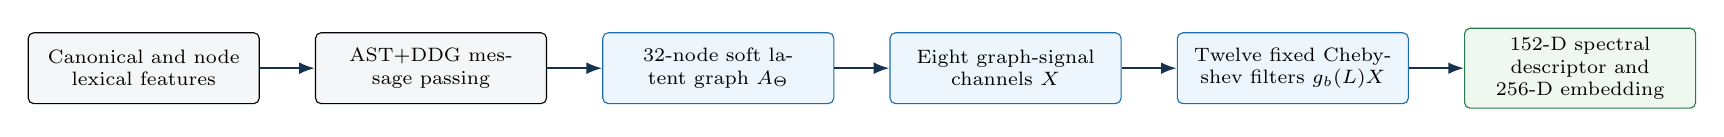
\begin{tikzpicture}[
  node distance=5mm and 7mm,
  box/.style={draw,rounded corners=2pt,align=center,minimum height=9mm,
    text width=27mm,font=\scriptsize,fill=lightgray},
  graph/.style={box,fill=lightblue,draw=blue},
  outputbox/.style={box,fill=lightgreen,draw=green},
  arr/.style={-{Latex[length=2mm]},thick,draw=navy}
]
\node[box] (input) {Canonical and node lexical features};
\node[box,right=of input] (gnn) {AST+DDG message passing};
\node[graph,right=of gnn] (latent) {32-node soft latent graph $A_\Theta$};
\node[graph,right=of latent] (signal) {Eight graph-signal channels $X$};
\node[graph,right=of signal] (filter) {Twelve fixed Chebyshev filters $g_b(L)X$};
\node[outputbox,right=of filter] (output) {152-D spectral descriptor and 256-D embedding};
\draw[arr] (input)--(gnn);
\draw[arr] (gnn)--(latent);
\draw[arr] (latent)--(signal);
\draw[arr] (signal)--(filter);
\draw[arr] (filter)--(output);
\end{tikzpicture}}
\caption{Every attribute-dependent output route crosses the learned graph and a
graph-spectral operator.}
\end{figure}

The learned soft weighted adjacency defines the normalized Laplacian
\begin{equation}
L=I-D^{-1/2}A_\Theta D^{-1/2}.
\end{equation}
Final latent states $Z'\in\R^{32\times256}$ are projected to eight graph-signal
channels and RMS-normalized:
\begin{equation}
X=\frac{Z'W_s}{\sqrt{\operatorname{mean}_v(Z'W_s)^2+\epsilon}}
\in\R^{32\times8}.
\end{equation}
Twelve Gaussian spectral bands are approximated by degree-12 Chebyshev
polynomials. Only permutation-invariant filtered energy is retained:
\begin{align}
Y_{bq}&=g_b(L)X_q,\\
e_{bq}&=\log\left(1+\frac{1}{32}\sum_{v=1}^{32}Y_{bq}(v)^2\right).
\end{align}
The final descriptor is
\begin{equation}
s=[\underbrace{d(\lambda)}_{32};
\underbrace{h(\lambda)}_{24};
\underbrace{\operatorname{vec}(e)}_{12\times8=96}]
\in\R^{152}.
\end{equation}

\begin{summarybox}{lightblue}{What is excluded}
There is no direct $\operatorname{mean}(Z')$, no source-token residual, and no
input-conditioned band-attention gate. Lexical information remains useful, but
its output effect must appear through $A_\Theta$, $L$, and $g_b(L)X$.
\end{summarybox}

\clearpage
\section*{3. What failed, and what the new run shows}

The first redesign exposed only 56 adjacency-spectrum statistics: 32 spectral
density values and 24 heat-trace values. This created the bottleneck
$X\rightarrow A_\Theta\rightarrow\lambda(L)$ and discarded most attributed
information. Fixed top-k sparsification also made latent graphs spectrally too
similar, while positive-F1 checkpoint selection could prefer all-positive
predictions on balanced data.

\begin{table}[H]
\centering
\small
\begin{tabular}{lrrrrrrr}
\toprule
AtCoder version & P & R & F1 & Acc & Macro-F1 & BA & AUC \\
\midrule
First redesign: adjacency-only & 0.500 & 1.000 & 0.667 & 0.500 & 0.333 & 0.500 & 0.498 \\
Second redesign: graph-signal & 0.795 & 0.872 & 0.832 & 0.824 & 0.823 & 0.824 & 0.893 \\
\bottomrule
\end{tabular}
\caption{The first method predicts every AtCoder pair as positive; the second
method restores genuine class separation.}
\end{table}

The new run uses all 544,054 training, 116,704 validation, and 116,736 test
pairs. The balanced test split contains 58,368 positives and 58,368 negatives.
Its confusion matrix is
\begin{equation}
TP=50{,}917,\quad FP=13{,}133,\quad TN=45{,}235,\quad FN=7{,}451.
\end{equation}
The predicted-positive rate is 0.5487 rather than 1.0. Probability standard
deviation is 0.4057 rather than a near-constant distribution. Because ROC-AUC
is 0.893, the improvement is not an artifact of threshold selection.

\begin{figure}[H]
\centering
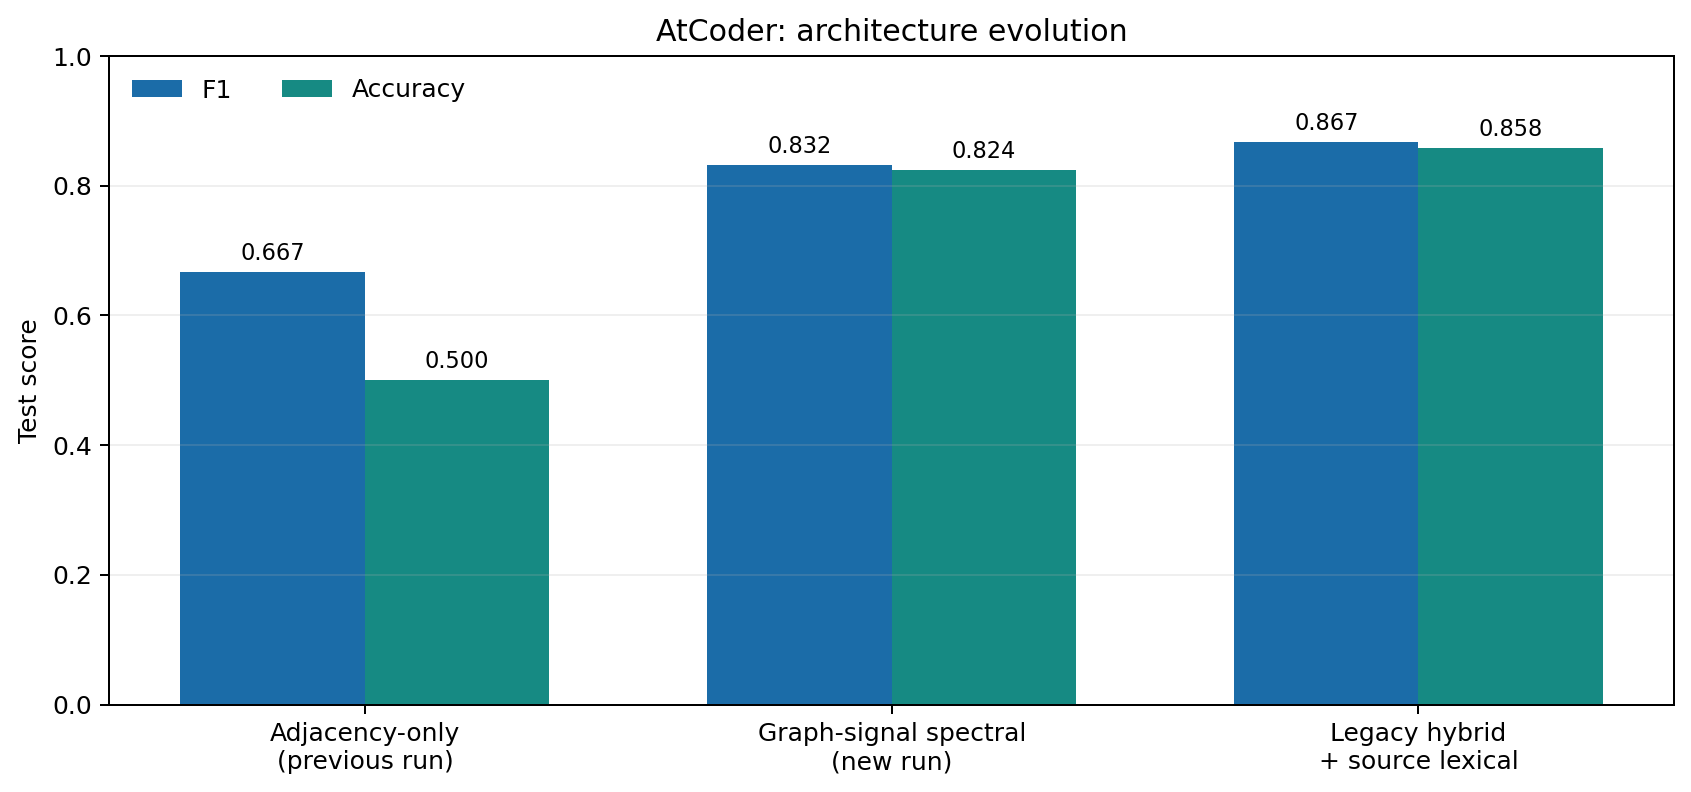
\includegraphics[width=0.87\linewidth]{assets/method_evolution/atcoder_method_comparison.png}
\caption{The new method recovers most legacy performance without restoring the
direct lexical bypass.}
\end{figure}

Relative to adjacency-only, the second redesign improves F1 by 0.165, Accuracy
by 0.324, Macro-F1 by 0.490, and ROC-AUC by 0.395. It recovers 82.5 percent of
the F1 gap and 90.4 percent of the Accuracy gap between adjacency-only and the
strongest historical hybrid configuration. It is 0.003 F1 above the historical
Graph + labels model without source lexical, but remains 0.035 F1 below the
best historical model that used a direct source-lexical residual.

\clearpage
\section*{4. Scientific interpretation and next decisions}

\begin{summarybox}{lightgreen}{Defensible conclusion}
The first redesign failed, but the latent graph-representation idea did not.
The second redesign demonstrates that semantic attributes can be retained
without an independent feature branch when they are treated as graph signals
and processed by spectral operators. The new AtCoder representation is useful,
non-collapsed, and methodologically aligned with an attributed graph-spectral
claim.
\end{summarybox}

\subsection*{What can be claimed now}
\begin{itemize}
\item Direct node-state and source-lexical bypasses are absent from the revised
readout.
\item Canonical and node lexical attributes influence both latent graph
induction and graph-signal response.
\item The new AtCoder run provides strong separation: F1=0.832,
Accuracy=0.824, Macro-F1=0.823, and ROC-AUC=0.893.
\item The second redesign removes the all-positive collapse observed in the
adjacency-only model.
\end{itemize}

\subsection*{What should not yet be claimed}
\begin{itemize}
\item Universal superiority over all hybrid models or external baselines.
\item That the entire improvement comes only from graph-signal energy.
\item A stable final performance estimate from one seed and four epochs.
\end{itemize}

Several changes were introduced together: graph-signal energy, soft weighted
adjacency, fixed bands, collapse-aware monitoring, and robust checkpoint and
threshold ordering. Controlled ablations are required to isolate them.

\subsection*{Highest-priority experiments}
\begin{enumerate}
\item Run the revised SemanticCloneBench notebook for its configured 30-epoch
schedule.
\item Train AtCoder beyond four epochs because validation AUC is still rising
and the best checkpoint is the final epoch.
\item Report at least three seeds, preferably five.
\item Compare adjacency-only, attributed graph-signal, hybrid latent, and
source-lexical arms under one locked protocol.
\item Perform Laplacian and signal dependence tests by perturbing $L$ and $X$
separately at evaluation time.
\end{enumerate}

\subsection*{Recommended one-sentence description}

SPECTRA-Siam maps each program to a learned weighted latent graph and constructs
its final embedding only from latent-spectrum summaries and permutation-invariant
energies of canonical and lexical node signals filtered on the learned graph,
without pooled node-state or source-token bypasses.

\vfill
\begin{center}
\small
Full technical report: \code{output/pdf/attributed\_graph\_spectral\_method\_comparison.pdf}
\end{center}

\end{document}
